

\documentclass[a4paper,12pt]{article}
%%%%%%%%%%%%%%%%%%%%%%%%%%%%%%%%%%%%%%%%%%%%%%%%%%%%%%%%%%%%%%%%%%%%%%%%%%%%%%%%%%%%%%%%%%%%%%%%%%%%%%%%%%%%%%%%%%%%%%%%%%%%%%%%%%%%%%%%%%%%%%%%%%%%%%%%%%%%%%%%%%%%%%%%%%%%%%%%%%%%%%%%%%%%%%%%%%%%%%%%%%%%%%%%%%%%%%%%%%%%%%%%%%%%%%%%%%%%%%%%%%%%%%%%%%%%
\usepackage{eurosym}
\usepackage{vmargin}
\usepackage{amsmath}
\usepackage{graphics}
\usepackage{epsfig}
\usepackage{subfigure}
\usepackage{fancyhdr}
%\usepackage{listings}
\usepackage{framed}
\usepackage{graphicx}

\setcounter{MaxMatrixCols}{10}
%TCIDATA{OutputFilter=LATEX.DLL}
%TCIDATA{Version=5.00.0.2570}
%TCIDATA{<META NAME="SaveForMode" CONTENT="1">}
%TCIDATA{LastRevised=Wednesday, February 23, 2011 13:24:34}
%TCIDATA{<META NAME="GraphicsSave" CONTENT="32">}
%TCIDATA{Language=American English}

\pagestyle{fancy}
\setmarginsrb{20mm}{0mm}{20mm}{25mm}{12mm}{11mm}{0mm}{11mm}
\lhead{Shiny} \rhead{Dublin \texttt{R}}
\chead{Formatting Text}
%\input{tcilatex}
\begin{document}

\subsection*{Formatted Text}

\begin{framed}
\begin{verbatim}
# ui.R

shinyUI(fluidPage(
  titlePanel("My Shiny App"),
  sidebarLayout(
    sidebarPanel(),
    mainPanel(
      p("p creates a paragraph of text. 
      Note: this paragraph is followed by br(), 
      which makes a blank line."),
      #------------------#
      p("A new p() command starts a new paragraph. 
      Supply a style attribute to change the format of the entire paragraph", 
      style = "font-family: 'times'; font-si16pt"),
      #------------------#
      strong("strong() makes bold text."),
      #------------------#
      em("em() creates italicized (i.e, emphasized) text."),
      br(),
      #------------------#
      code("code displays your text similar to computer code"),
      #------------------#
      div("div creates segments of text with a similar style. 
      This division of text is all blue because I passed the argument 
      'style = color:blue' to div", style = "color:blue"),
      #------------------#
      br(),
      #------------------#
      p("span does the same thing as div, but it works with",
        span("groups of words", style = "color:blue"),
        "that appear inside a paragraph.")
    )
  )
))
\end{verbatim}
\end{framed}
\newpage

\begin{figure}[h!]
\centering
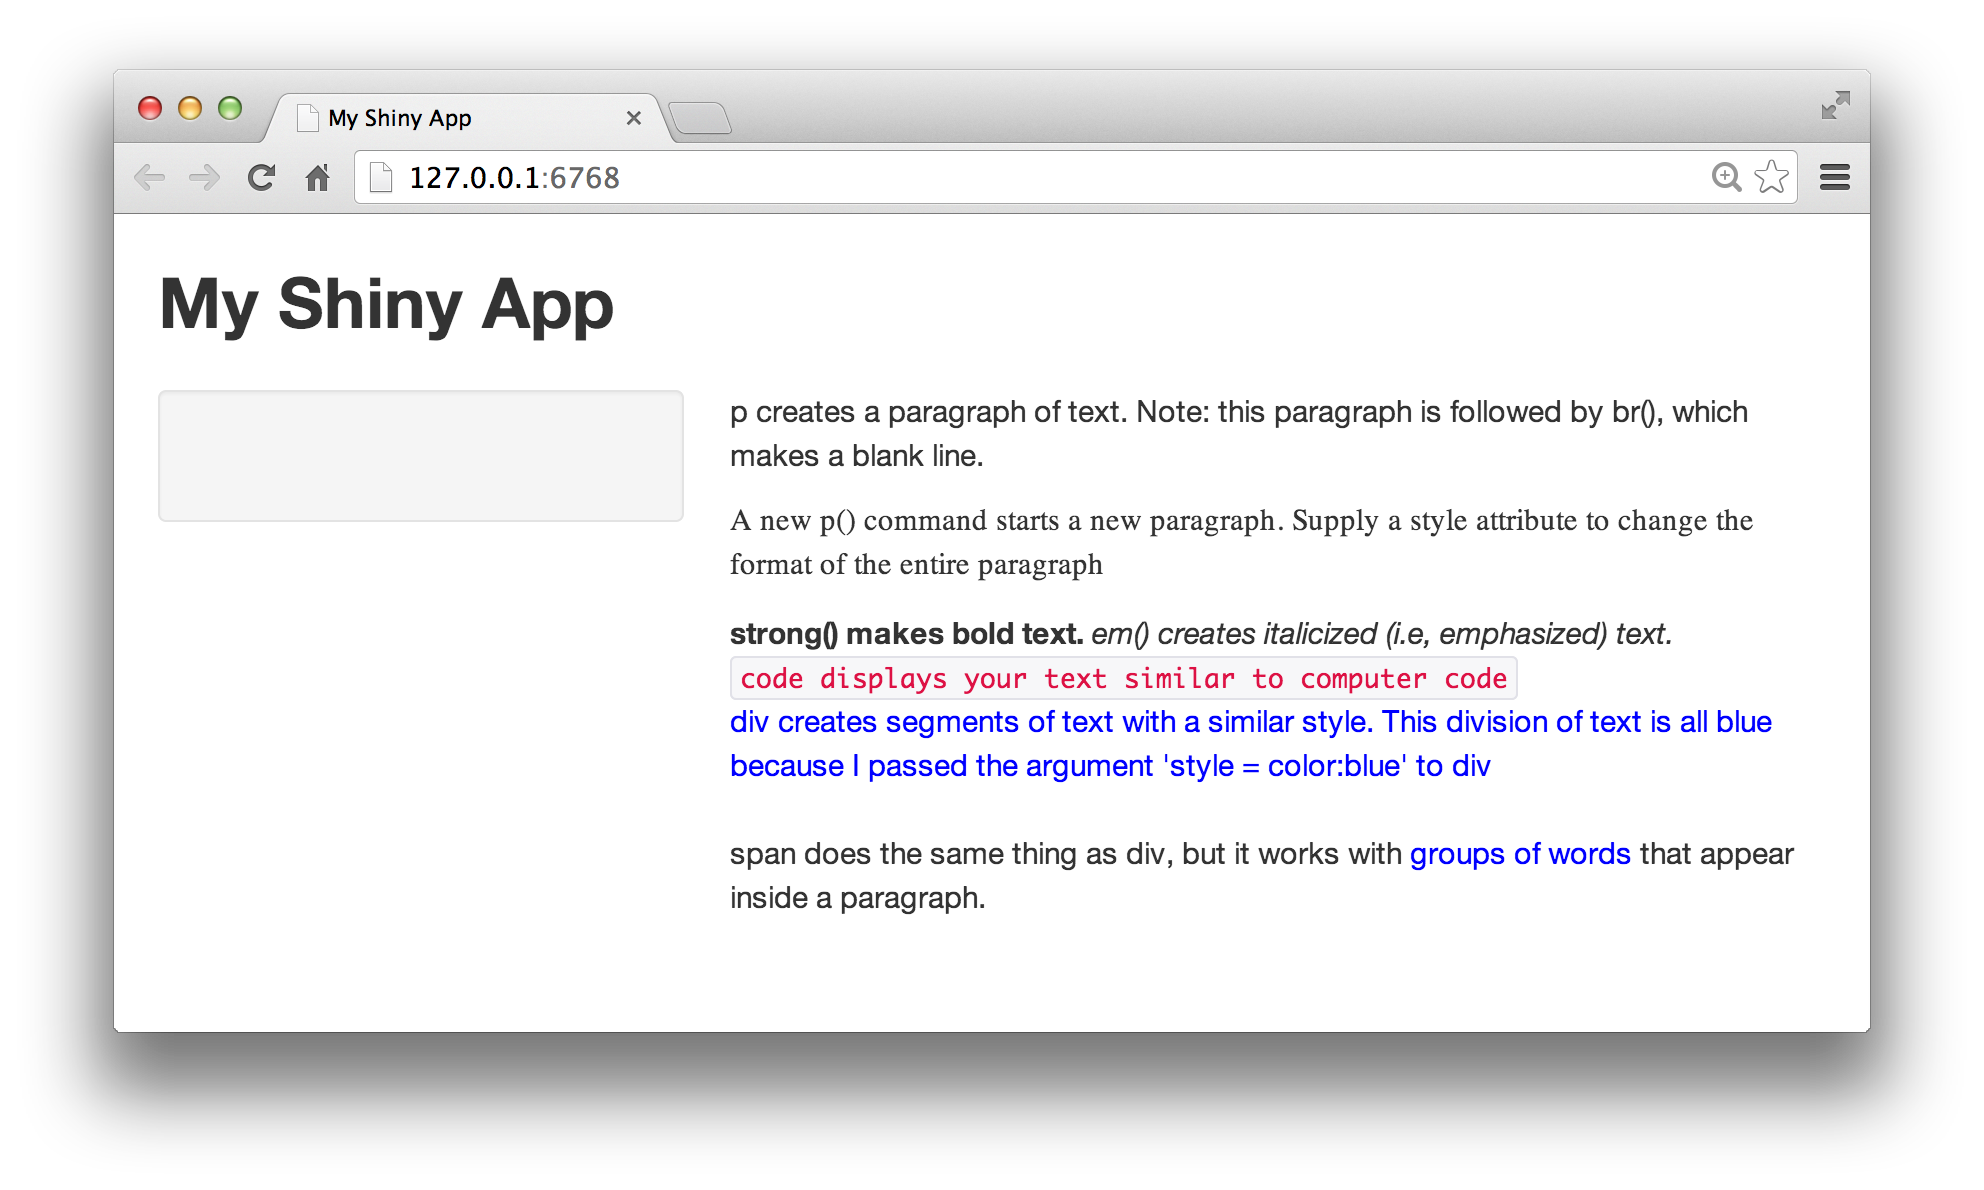
\includegraphics[width=0.99\linewidth]{./formatting}
\caption{}
\label{fig:formatting}
\end{figure}

\end{document}
